\documentclass[11pt]{article}
\usepackage{acl2014}
\usepackage[utf8]{inputenc}
\usepackage{times}
\usepackage{url}
\usepackage{amsmath}
\usepackage[natbib=true,backend=bibtex,style=authoryear,language=english]{biblatex}
\usepackage{lipsum}
\usepackage{latexsym}
\usepackage[normalem]{ulem}
\usepackage[ruled]{algorithm2e}
\usepackage[]{setspace}
\useunder{\uline}{\ul}{}
\usepackage{caption} 
\usepackage{lastpage}
\usepackage{float}
\usepackage[page]{appendix}
\pagestyle{plain} 
\usepackage{graphicx}
\captionsetup[table]{skip=10pt}
\title{Reinforcement Learning in Latent Space}

\addbibresource{../references.bib}
\AtBeginBibliography{\small}

\author{We, the authors}
  
\begin{document}

\maketitle
\begin{abstract}

\lipsum[1]

{{\it \bf Keywords: transfer learning, reinforcement learning}}
\end{abstract}
 
\section{Introduction}
\label{sec:introduction}

% topic introduction & motivation
Reinforcement learning (RL) addresses machine learning problems where complex tasks with minimal feedback \citep{taylor2007cross} need to be solved by agents in a sequence of actions as reactions to a changing environment. RL methods were successfully applied in different areas such as game playing \citep{silver2016mastering}, robotics \citep{levine2016end} and resources management \citep{mao2016resource}. 
Common approaches to RL create task-specific solutions. This means that when facing a new environment, the agent needs to restart learning. This limitation calls for transfer learning, which aims at transferring previously gained knowledge across different tasks. Besides reducing time-consuming re-training of similar tasks, transfer learning can potentially enable RL agents to operate in environments where learning is otherwise too challenging \citep{barreto2018transfer} or expensive. In RL, transfer faces two key challenges. Firstly, even if tasks are similar, state and action spaces may be of \textit{different dimensions} between them. Secondly, the agent's policy needs to be not \textit{overfitted} to the source task, in order to make the underlying knowledge reusable. % example pathing?
The first issue can be solved by only taking information into account that is available in all tasks, such as pixels. In fact, this is a rather obvious requirement: The agent can only learn transferable knowledge, if it is presented with information that allows it to find common patterns. The second problem, learning generalizable policies, is more challenging and requires models that guide the agent towards a transferable policy. 

% approach
In this work, we explore the possibility of using a latent representation created by a deep neural network to achieve transfer learning in RL. Deep learning methods can discover representations that are abstract and domain-invariant \citep{bengio2012deep, ganin2014unsupervised}. This characteristic can be utilized for transfer learning in RL. Instead of presenting the agent with the raw state of an environment, a representation module first encodes the pixels into a latent space using a stack of convolutional layers. In contrast to previous research \citep[see e.g.][]{DQN, DuelingDQN}, we not only train this representation on the given task but also calculate the loss using an autoencoder architecture. This guides the encoder into creating representations that can be used to reconstruct the given image. We hypothesize such representations to encode important features in the resulting latent space and therefore make it easier to generalize to new tasks.

% research questions & contributions
More specially, we seek to answer the following research questions:
\begin{itemize}
	\item Can the proposed autoencoder architectures capture commonalities of several similar yet different tasks, such that an RL agent can use the encoded representation to learn to perform all these tasks?
	\item After learning a task based on the encoded representation, can the agent learn to perform a previously unseen but similar task more easily (e.g. taking less time to train)? Or can the agent do so without learning?
\end{itemize}

% outlook
In the following sections, we first review selected previous works relevant to our approach. We then introduce our own model and describe the different techniques used in the final system in detail (Section \ref{sec:approach}). In Section \ref{sec:experiments} the experimental setup is described, followed by the results in Section \ref{sec:results}. We discuss these results in Section \ref{sec:discussion} and finally draw a conclusion.
%!TEX root = ../report.tex

\section{Approach}
\label{sec:approach}
In this work, we propose a modular framework for transfer learning in reinforcement learning. 
This framework consists of three modules: 
\begin{enumerate}[i]
    \item the \textbf{representation module}, which constructs an abstract representation of the task environment;
    \item the \textbf{policy learner}, which is a RL learner operating based on the task abstraction created by the representation module;
    \item the \textbf{task environment}, which is the RL task to be solved by the policy learner.
\end{enumerate}
In the following we first present the representation module and the policy module and then depict their interplay in the agent's parallel learning process. The tasks that these different modules are tested on will be introduced in Section \ref{sec:experiments}.

\subsection{Representation Module}
The representation module aims at constructing an abstract and useful generalized representation of the environment's states to facilitate later knowledge transfer. In this work, several architectures are proposed as visualized in Figure \ref{fig:repr_learner} and described in the follwoing subsections. All these architectures follow the pattern of an autoencoder \citep{ballard1987modular} and include some lower-dimensional ``bottleneck'' layers for dimensionality reduction of the input. Autoencoders have shown before to be useful for learning representations \citep{bengio2012deep} in different applications (see e.g. \citet{ap2014autoencoder} and \citet{silberer2014learning} for language or \citet{wang2013learning} for images). We will use the middle layer representation as the latent space projection on which the DDQN learns its policy.
Once learned, this intermediate latent space is expected to create a more compact and abstract representation of the original environment and serve as the basis of transfer learning. This is opposed to previous work that trained the convolutional layers only on the loss produced by the DQN (or, more generally, the policy). We hypothesize the generality of the latent space guided by the representation module to help when transferring knowledge. 

In the following, we will refer to the error calculated based on the heads of the architectures presented below as the \textit{autoencoder loss}. This is to be distinguished from the \textit{policy loss} that is referring to the error calculated by the DDQN.

\begin{figure}[ht!]
	\centering
	\begin{subfigure}{0.45\columnwidth}
		\centering
		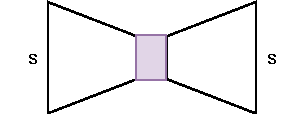
\includegraphics[width=\linewidth]{img/very_simple_autoencoder.pdf}
		\caption{Simple autoencoder}
		\label{subfig:repr_learner_simple_autoencoder}
	\end{subfigure}%
	~ 
	\begin{subfigure}{0.45\columnwidth}
		\centering
		\includegraphics[width=\linewidth]{documentation/report/img/variational_autoencoder_ver2.png}
		\caption{Variational autoencoder}
		\label{subfig:repr_learner_vae}
	\end{subfigure}
	\begin{subfigure}{0.5\columnwidth}
		\centering
		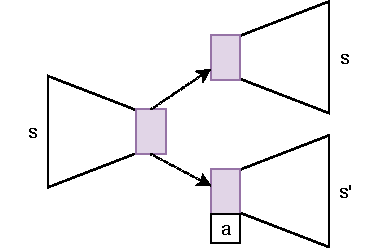
\includegraphics[width=\linewidth]{img/janus.pdf}
		\caption{Janus}
		\label{subfig:repr_learner_janus}
	\end{subfigure}%
	~ 
	\begin{subfigure}{0.5\columnwidth}
		\centering
		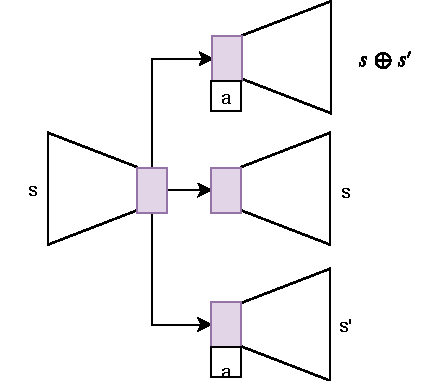
\includegraphics[width=\linewidth]{img/cerberus.pdf}
		\caption{Cerberus}
		\label{subfig:repr_learner_cerberus}
	\end{subfigure}
	\caption{Network architectures of different representation modules, where $s$ and $s'$ indicate current and next state respectively, and $a$ indicates the action leading from $s$ to $s'$. 
	The layers marked in purple are the latent representations to be used as the basis of later transfer learning. 
	The arrows indicate a straight copy from source to target.
	}
	\label{fig:repr_learner}
\end{figure}

\subsubsection{Simple and Variational Autoencoder}
The simplest representation module is the classic autoencoder, which in our case compresses and reconstructs the current state. Figure \ref{subfig:repr_learner_simple_autoencoder} illustrates the \textit{simple autoencoder}.  A modification to this basic model is the so called variational autoencoder (VAE) (see Figure \ref{subfig:repr_learner_vae}). A VAE is a generative approach that models the latent distribution with a Gaussian distribution. Whether it is the simple or variational autoencoder, one theoretical drawback of using such a simple structure for representation learning is that since the latent space only aims at compressing the state and no dynamics of the task are encoded, it is not necessarily a useful basis for learning a policy. The upcoming architectures aim to account for this.

\subsubsection{Janus}
To create more guidance in the construction of the latent space, we add another decoder to capture the dynamics of the environment. As shown in Figure \ref{subfig:repr_learner_janus}, in addition to reconstructing the current state, we also append the action to the representation and seek to use this combination to predict the next state.
The hypothesized effect of this approach is that the latent representation is incentivized to preserve transition dynamics in the environment, and therefore is a more meaningful abstraction of the task.

\subsubsection{Cerberus}
Extending Janus, the Cerberus architecture adds another decoder, which aims at predicting the difference between the current and the next state. By predicting the differences instead of the next state in its entirety, focus is placed on the change caused by the action taken but also the dynamics of the environment in general. We expect this to be especially useful when the changes between consecutive states are small relative to the entire state representation. Optimally, this makes it easier for the encoder to focus on dynamic properties of the environment, such as the position of the agent. The network architecture is shown in Figure \ref{subfig:repr_learner_cerberus}.\\

While it is possible to use both Janus and Cerberus as variational autoencoders, experiments with the simple VAE showed that its representation is most likely too imprecise given the noisy nature of its latent space.

\subsection{Policy Learner}
Based on the latent space constructed by the representation module, the policy learner trains an RL agent to complete a given task. 
%One of the drawbacks of table-based Q-learning occurs in environments with large state spaces. Maintaining and updating the values of all possible states is memory intensive and requires a great amount of training data. An alternative that avoids this problem is function approximation, where Deep-Q-Networks are a popular algorithm.
We use the Double Deep Q-Network \citep{DDQN} algorithm, which is a Q-learning algorithm that uses deep neural networks to approximate the state Q-values of each action.

With the goal of improving and accelerating the learning process, experience replay \citep{replay_memory_oc} is used in conjunction with the algorithm. This mechanism stores the situations that the agent previously encountered as ``memories'' and randomly samples them to train the network. The sampling of memories is meant to remove correlation between training instances and avoid forgetting previous experiences, facilitating learning.

\subsection{Parallel Learning Process}
During training, the agent learns the construction of the latent space and the policy based on the latter in a parallel approach. In each step of every training episode, first the representation module is trained on a batch of observations. Subsequently, the DDQN is updated based on a state-action-reward-state tuple in which the states were encoded into the latent space using the new version of the representation module. 

\paragraph{Batch Representation Learning} To improve the efficiency of training the representation module, batch learning is used. All observations are stored in memory and are fed into the representation network in minibatches of size 32, randomly sampled from this memory. The memory is limited in its size to 1024 observations and dequeues in a \textit{first-in-first-out} manner.

\paragraph{Full backpropagation} Furthermore, when updating the policy, the loss of the DDQN is also backpropagated through the encoder of the representation module. This additionally biases the representation to be sensible to the collected rewards.\\

A parallel approach to learning the two submodules of the agent implicates that during early episodes, the latent states seen by the DDQN are of very low quality. To counteract this, the training involves a warm up period in which the DDQN learns only on single samples without storing them in a memory. Only after a chosen amount of steps the replay memory is going to be filled, assuming that the quality of the memories is now sufficient.

\paragraph{Multi-Task Learning} In multi-task learning, the training alters between the tasks by randomly choosing the next environment at the beginning of each episode. If the observations are given to the DDQN in the same order, this could lead to the agent constantly trying to perform well in the new task, instead of finding a general policy. As a solution we propose an experience stack in which each experience (that is, a state-action-reward-state tuple and the done-flag) is stored when observed. After a warm up period that fills the stack, at each step a random element is popped from the stack and fed to the policy.

\paragraph{Intergradient Learning Phases} In the beginning of training, efficient learning of a useful representation is crucial. In later stages, the representation should only be fine-tuned, since the policy needs to see consistent input. Additionally, the training based on the auto-encoder's loss is supposed to guide the encoder towards representing a generalizable latent space. But when progressing, this guidance should slowly diminish to allow the DDQN to fine-tune the encoder to task-oriented needs. We guarantee such an intergradient learning by introducing a learning rate schedule to the representation module that reduces the learning rate of the auto-encoder by 10 percent every 500 episodes. At the same time the learning rate of the DDQN is kept constant. To speed up learning, we heuristically set 500,000 episodes to be the point at which the learning rate is so small that we can turn off updating based on the autoencoder loss. 

\begin{figure*}[t]
	\centering
	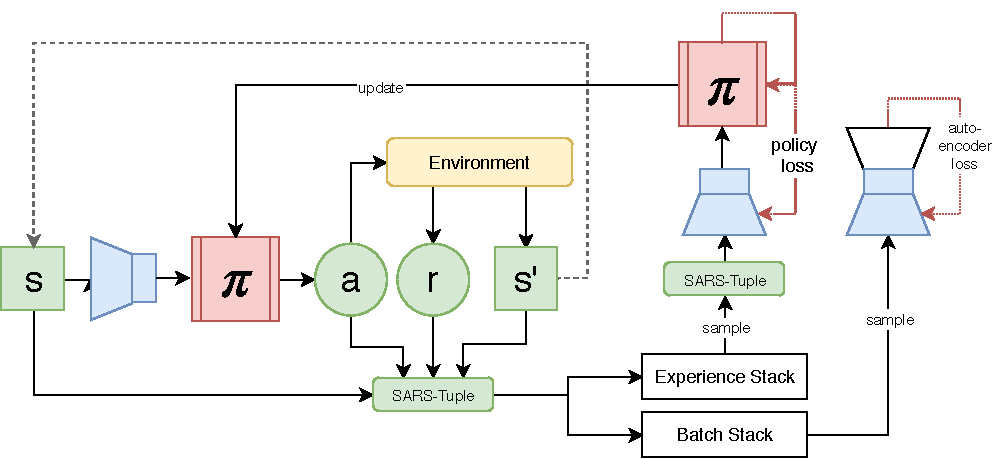
\includegraphics[width=\textwidth]{img/full-model.pdf}
	\caption{Illustration of the parallel approach, where the representation module and policy are trained simultaneously as the agent operates in the environment. At every time step, the current state is given to the current version of the representation module's \textit{encoder} (blue). The resulting latent space representation is used by the current policy (red) to decide on the best action. After executing this action, the environment gives back an immediate reward and the next state. The four-tuple of current state \textit{s}, action \textit{a}, reward \textit{r} and next state \textit{s'} (green) is stored in both an experience stack and a batch stack. From the experience stack, one random tuple is sampled and fed into representation module and subsequently the policy, where a policy loss is calculated and backpropagated through both the DDQN (policy) and the representation module's encoder. This updates the policy used in the next iteration. Furthermore, a batch of 32 tuples is sampled from the batch stack and fed through the full representation module to calculate an autoencoder loss that is backpropagated through the full representation module. Finally, the next state is taken as the current state and the procedure repeats itself. \label{fig:approaches}}
\end{figure*}

% \subsubsection{History Approach}
% As the name indicates, the history approach first creates a collection of states, actions and rewards by randomly exploring in the environment.
% The representation module is then trained based on the collected history.
% Once learning completes, the policy learner is trained based on the encoding of the representation module.
% In this approach, the representation and policy learning are sequential and decoupled. 
\section{Tasks \& Experiments}
\lipsum[2-3]

%\section{Results}
\label{sec:results}

In the following, we report and analyze the results of the experiments described in the previous section. 

\subsection{Representation Modules}

\subsubsection{Decoder Output}
We begin by qualitatively analyzing the reconstructions created by the variational autoencoder (VAE), the Janus architecture and the Cerberus architecture. Note that while we will loosely refer to the outputs of the decoders as \textit{reconstructions} in the following, only the leftmost output of the multi-decoder architectures is an actual reconstruction. As described in Section \ref{sec:approach}, the middle and right output are predictions or approximations of unseen information.

\begin{figure}[t!]
	\centering
	\begin{subfigure}{0.6\columnwidth}
		\centering
		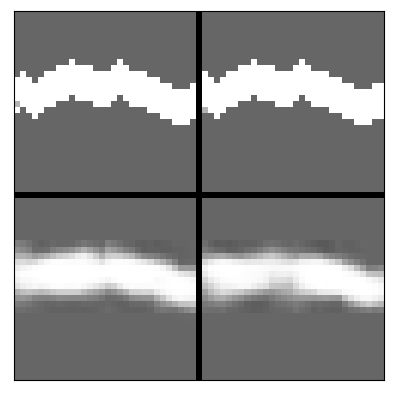
\includegraphics[width=\linewidth]{img/janus_tunnel_recon.png}
		\caption{Janus. Left is the current frame, right is the next frame.}
		\label{subfig:janus_reconstruction}
	\end{subfigure}%
	~ 
	\begin{subfigure}{0.3\columnwidth}
		\centering
		
\includegraphics[width=\linewidth]{img/cvae_tunnel_recon.png}
		\caption{CVAE.}
		\label{subfig:cvae_reconstruction}
	\end{subfigure}
	
	
	\begin{subfigure}{0.9\columnwidth}
		\centering
		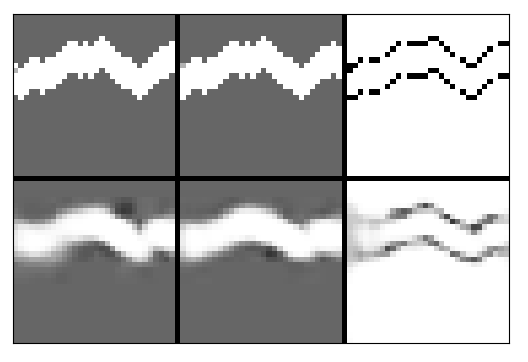
\includegraphics[width=\linewidth]{img/cerberus_tunnel_recon.png}
		\caption{Cerberus. From left to right are the current frame, next frame, and the differences between the two frames.}
		\label{subfig:cerberus_reconstruction}
	\end{subfigure}

	\caption{Reconstruction of the different representation learners performing over the Tunnel task. For each architecture the ground-truth (upper images) and the reconstructions (lower images) are depicted.}
	\label{fig:repr_learner_reconstructions}
\end{figure}

Figures \ref{fig:repr_learner_reconstructions} to \ref{fig:cvae_multitask} show examples of the outputs of the decoders in the three different architectures. Figure \ref{fig:repr_learner_reconstructions} is the result of 500,000 episodes of training on the Tunnel task. It comes unsurprising that the reconstructions are not perfect, since the environment is randomly generated. Out of the three architectures, Janus seems to be most flawed. Although the course of the tunnel seems correctly reconstructed, its borders are a lot blurrier. The CVAE appears to reconstruct slightly more defined borders and also approximates the tunnel's course well. Similarly, Cerberus produces borders that are more clearly defined than in Janus.

% CVAE MT
\begin{figure}[t!]
	\centering
	\begin{subfigure}{0.3\columnwidth}
		\centering
		
\includegraphics[width=\linewidth]{documentation/report/img/cvae_scroll_evasion.png}
		\caption{Evasion.}
		\label{subfig:cvae_scroll_race}
	\end{subfigure}%
	~ 
	\begin{subfigure}{0.3\columnwidth}
		\centering
		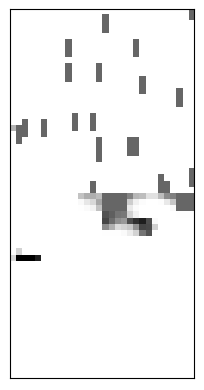
\includegraphics[width=\linewidth]{documentation/report/img/cvae_scroll_walls.png}
		\caption{Wall Evasion.}
		\label{subfig:cvae_scroll_walls}
	\end{subfigure}
	~ 
	\begin{subfigure}{0.3\columnwidth}
		\centering
		
\includegraphics[width=\linewidth]{documentation/report/img/cvae_scroll_tunn.png}
		\caption{Tunnel.}
		\label{subfig:cvae_scroll_tunnel}
	\end{subfigure}

	\caption{Reconstruction of CVAE trained on multiple scroller tasks (Race, Walls Evasion and Tunnel). For each task the ground-truth (upper images) and the reconstructions (lower images) are depicted.}
	\label{fig:cvae_multitask}
\end{figure}

% JANUS MT
\begin{figure}[t!]
	\centering
	\begin{subfigure}{0.3\columnwidth}
		\centering
		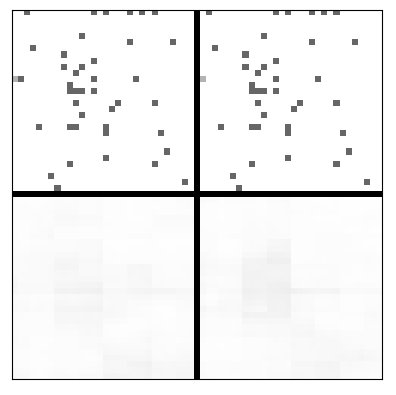
\includegraphics[width=\linewidth]{documentation/report/img/janus_scroll_evasion.png}
		\caption{Evasion.}
		\label{subfig:janus_scroll_race}
	\end{subfigure}%
	~ 
	\begin{subfigure}{0.3\columnwidth}
		\centering
		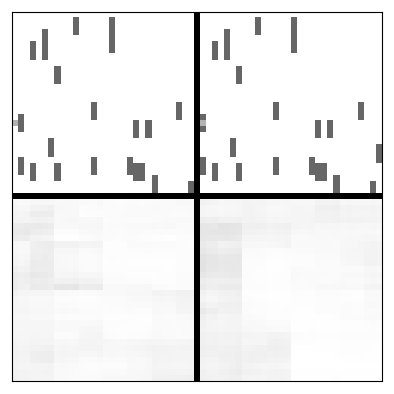
\includegraphics[width=\linewidth]{documentation/report/img/janus_scroll_walls.png}
		\caption{Wall Evasion.}
		\label{subfig:janus_scroll_walls}
	\end{subfigure}%
	~ 
	\begin{subfigure}{0.3\columnwidth}
		\centering
		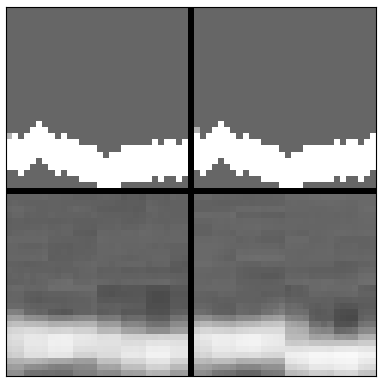
\includegraphics[width=\linewidth]{documentation/report/img/janus_scroll_tunnel.png}
		\caption{Tunnel.}
		\label{subfig:janus_scroll_tunnel}
	\end{subfigure}

	\caption{Reconstruction of Janus trained on multiple scroller tasks (Race, Wall Evasion and Tunnel). For each task the ground-truth (upper images) and the reconstructions (lower images) are depicted.}
	\label{fig:janus_multitask}
\end{figure}


% CERBERUS MT 
\begin{figure}[t!]
	\centering
	\begin{subfigure}{0.3\columnwidth}
		\centering
		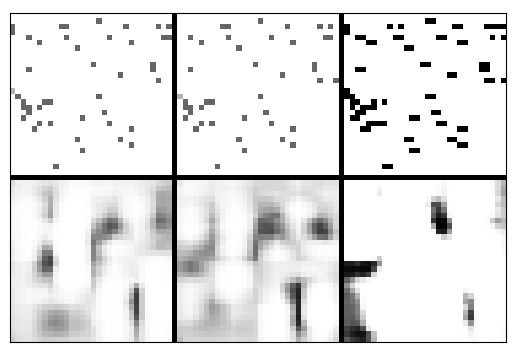
\includegraphics[width=\linewidth]{documentation/report/img/cerb_scroll_evasion.png}
		\caption{Evasion.}
		\label{subfig:cerberus_scroll_race}
	\end{subfigure}%
	~ 
	\begin{subfigure}{0.3\columnwidth}
		\centering
		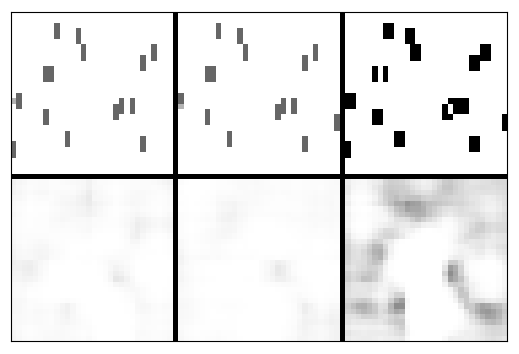
\includegraphics[width=\linewidth]{documentation/report/img/cerb_scroll_walls.png}
		\caption{Wall Evasion.}
		\label{subfig:cerberus_scroll_walls}
	\end{subfigure}
	~ 
	\begin{subfigure}{0.3\columnwidth}
		\centering
		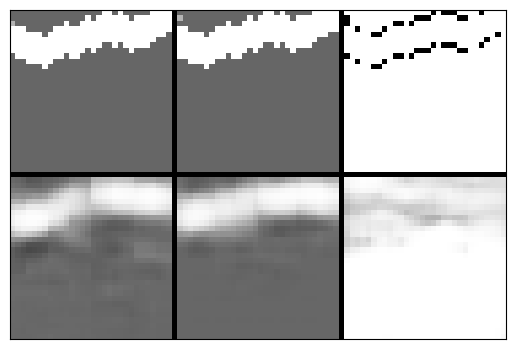
\includegraphics[width=\linewidth]{documentation/report/img/cerb_scroll_tunn.png}
		\caption{Tunnel.}
		\label{subfig:cerberus_scroll_tunnel}
	\end{subfigure}

	\caption{Reconstruction of Cerberus trained on multiple Scroller tasks (Race, Wall Evasion and Tunnel). For each task the ground-truth (upper images) and the reconstructions (lower images) are depicted.}
	\label{fig:cerberus_multitask}
\end{figure}

In Figures \ref{fig:cvae_multitask}, \ref{fig:janus_multitask} and \ref{fig:cerberus_multitask} the performance of CVAE, Janus and Cerberus is shown resulting from a multi-task learning on the Scroller tasks. The added challenge of reconstructing different environments makes the quality of the decoding decrease. For all architectures, the Tunnel is at least placed in the correct parts of the environment. Note though, that this is useless information for the agent, when performing the task since the position of the tunnel is irrelevant for the agent's relative position inside it. The course is rudimentally approximated by CVAE and Cerberus, but Janus experiences even more difficulties with this. The Evasion and Wall Evasion environment are a bigger challenge. This comes unsurprising, since the placement of obstacles is entirely random while the Tunnel forms a continuous entity. Interestingly, the CVAE's reconstructions in these tasks seem to be entirely unrelated to the input. For Evasion, no structure can be observed. The Wall Evasion reconstruction contains structure, but without any obvious connection to the input state. Janus produces reconstructions with slightly more structure than the CVAE Evasion reconstruction for both Evasion and Wall Evasion. Only in the case of Evasion there is a visible connection between the input and output: The area where pixels are densely agglomerated in the input is shaded darker in the reconstruction. Cerberus produces structure with the most contrast in its reconstructions for Evasion and Wall Evasion. For both tasks, the reconstruction is very imprecise, but white areas seem to resemble empty areas of the input.

We attribute the ability of Cerberus to reconstruct sharper edges than Janus to the difference-decoder forcing the reconstruction to pay more attention to the contours.

Due to the undesirable performance of CVAE and the limited computation power, we do not include it in further experiments.
%Since CVAE seems to struggle most with the multi-task setting and our time and computation power resources are limited, we will exclude it from the full system experiments.

\subsubsection{Latent Space Analysis}
\begin{figure}[t!]
	\centering
	\begin{subfigure}{0.46\columnwidth}
		\centering
		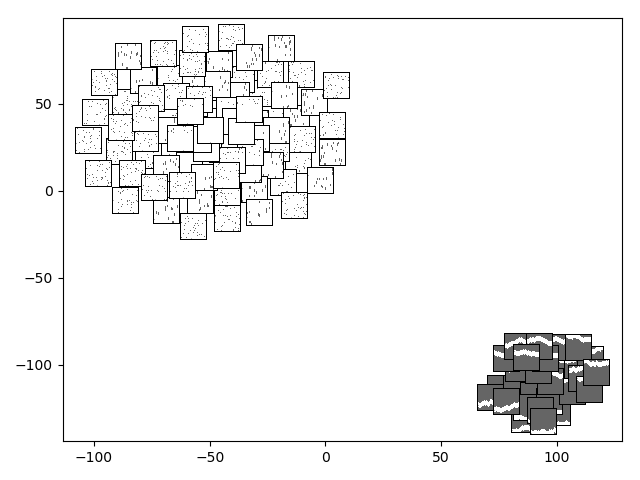
\includegraphics[width=\linewidth]{documentation/report/img/scroller_state.png}
		\caption{t-SNE on raw states.}
		\label{subfig:tsne_multitask_states}
	\end{subfigure}%
	~ 
	\begin{subfigure}{0.46\columnwidth}
		\centering
		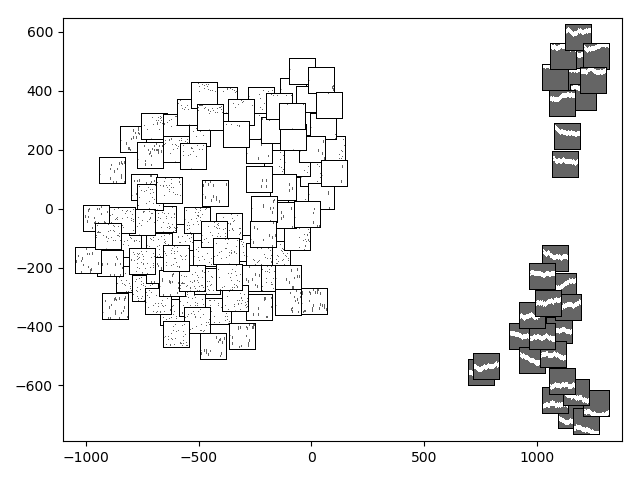
\includegraphics[width=\linewidth]{documentation/report/img/scroller_latent.png}
		\caption{t-SNE on latent states.}
		\label{subfig:tsne_multitask_latent}
	\end{subfigure}

	\caption{t-SNE projections in the multitask environment.}
	\label{fig:tsne-multitask}
\end{figure}

\begin{figure}[t!]
	\centering
	\begin{subfigure}{0.46\columnwidth}
		\centering
		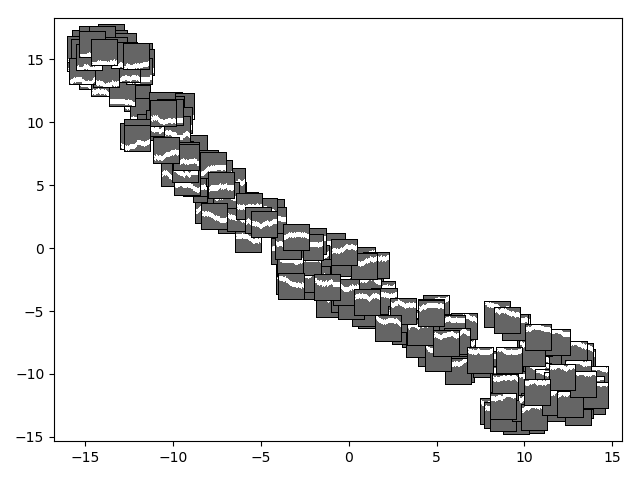
\includegraphics[width=\linewidth]{documentation/report/img/tunnel_state.png}
		\caption{t-SNE on raw states.}
		\label{subfig:tsne_tunnel_states}
	\end{subfigure}%
	~ 
	\begin{subfigure}{0.46\columnwidth}
		\centering
		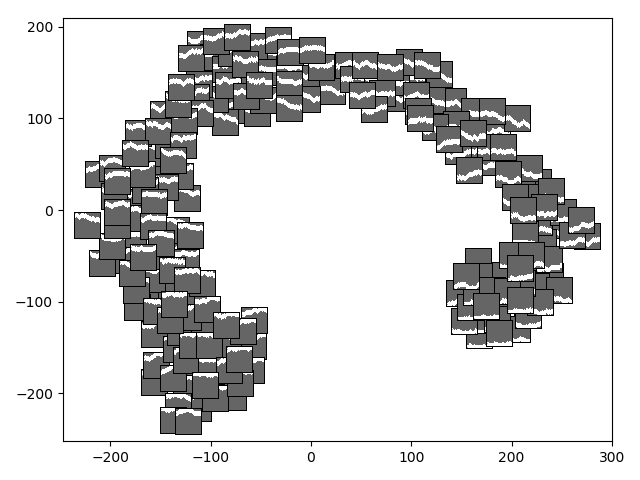
\includegraphics[width=\linewidth]{documentation/report/img/tunnel_latent.png}
		\caption{t-SNE on latent states.}
		\label{subfig:tsne_tunnel_latent}
	\end{subfigure}

	\caption{t-SNE projections in the Tunnel environment.}
	\label{fig:tsne-tunnel}
\end{figure}

To inspect the latent representations constructed by the encoders, we visualize the encoded states from different tasks with t-Distributed Stochastic Neighbor Embedding (t-SNE) \citep{tsne}. 

\paragraph{Latent Space of Multiple Tasks}
Figure \ref{fig:tsne-multitask} shows the original states and the latent states respectively with their dimensionalities reduced to two. Thirty states are sampled from each of Evasion, Wall Evasions, and Tunnel. 
As t-SNE preserves relative distances in high dimensional spaces, the frames closer to each other in the visualizations tend to be closer in the original spaces too.

In Figure \ref{subfig:tsne_multitask_states}, the original 30*30 input are plotted on two dimensions.
As expected, frames from Tunnel form their own cluster far apart from those from other tasks due to their distinct spatial characteristic, namely the large continuous areas of dark pixels. One can further observe that the nearly-empty frames are closer to each other, forming the center of the lower-left cluster.
This center is surrounded by other frames containing more dark pixels.

The t-SNE output in Figure \ref{subfig:tsne_multitask_latent} is based on the encoded latent states, although only the original frames are plotted to aid visual interpretation.
Unlike previously, the embedding clearly distinguishes the frames with dense dark pixels from those without. It furthermore shows a smooth gradient corresponding to the change in dark pixel density.
This provides evidence that the latent representation is able to capture abstract features of the inputs.
However, the frames from Tunnel still fall far from the other tasks, indicating that the encoder has not found a common representation for all tasks.
It is also visible that there is a further separation of Tunnel frames based on their spatial arrangements, i.e. the positions of the tunnels.

\paragraph{Latent Space of Tunnel Task} \label{para:latent_tunnel}
When using the representation module trained only on Tunnel and projecting latent spaces from Tunnel using t-SNE (Figure \ref{fig:tsne-tunnel}), a key problem of our approach becomes apparent. 
The additional structure in the Tunnel environment reveals the encoders inability to identify information relevant to tasks, that is, local information around the agent for these tasks. 
%Instead, the latent space is separating based on general structure.
Instead, the latent space is constructed based on the spatial structure of the frame, that is, the positions of the tunnel.
%In the case of the tunnel frames, this shows in the position of the tunnel in the frame being indicative of the latent space distance between states. 
As Figure \ref{subfig:tsne_tunnel_states} shows, this is the case without any latent state transformation as well. 

The curved structure in Figure \ref{subfig:tsne_tunnel_latent} could indicate that the latent space finds similarities between frames that would be more similar when horizontally mirrored.
However, this information is not useful for the agent when learning the task. In fact, the latent space should be grouping the frames based on the course of the tunnel and the current position of the agent. 

\subsection{Policy Learner}
The results for the different tasks were taken from a point during a 50,000 episode training where intermediate performance was maximal. This avoids taking the policy in a state where the agent currently reconsiders its solution to potentially find a better one.

Table \ref{tab:isolated_policy_learner} shows the performance of the DDQN on four tasks respectively. 
Note that the autoencoder weights are not updated by its own loss in order to test the policy learner in isolation.
On Pathing, Race, and Evasion, the performance is close to maximal and significantly outperform the random baselines.
However, in the Tunnel task the DDQN fails to learn an effective policy.
Its resulting behavior is simply a straight horizontal movement without any action initiated by the agent itself.

Since the effectiveness of the policy learner is proven on other tasks, we hypothesize that the poor performance is due to the latent representation not capturing useful information for this particular task.
The previous analysis of the latent space structure in Section \ref{para:latent_tunnel} provides further support for this hypothesis.
As previously stated, Figure \ref{subfig:tsne_tunnel_latent} shows that the latent representations for horizontally mirrored states are closer to each other. 
This contradicts the intuition that the learned representation should capture information about edge avoidance and therefore place such frames far apart.
%The fact that even the original DDQN without our modification cannot learn to do this trained on Tunnel alone (compare Table \ref{tab:isolated_policy_learner}) indicates the challenges posed by this task. 
But this observation also underlines the general difficulty of balancing between focusing on task-relevant features and generalizing for transfer learning.


\begin{table}[t!]
\centering
\begin{tabular}{@{}lllll@{}}
\toprule
\textbf{Task} & \textbf{$\mu_r$} & \textbf{$\widetilde{r}$} & \textbf{$\sigma_r$} & \textbf{baseline} \textbf{$\mu(r)$} \\ \midrule
Pathing & $-480$ & $-480$ & $0$ & $-8988$ \\
Race & $4103.6$ & $5000$ & $1783.8$ & $472$ \\
Evasion & $3949.7$ & $5000$ & $1543.7$ & $487.89$ \\
Tunnel & $193$ & $140$ & $313.06$ & $120$\\ 
\bottomrule
\end{tabular}
\caption{Performance of the DDQN without autoencoder loss but using a convolutional encoder. Results are given as arithmetic mean $\mu_r$ and median $\widetilde{r}$ over 100 test episodes. Baselines are random policies and therefore the absolute minimum performance. For the Race, Evasion and Tunnel task, maximum performance is 5000, while for Pathing -480 is the best score achievable.}
\label{tab:isolated_policy_learner}
\end{table}

% FINAL TEST ON TRANSFER
\subsection{Full System Experiments}
After performing individual experiments over the modules, we decided to not include the Convolutional Variational Autoencoder in the final experiments, being the representation module that performed worse, especially in a multi-task context.

\subsubsection{Zero-shot}
In Table \ref{zero-shot-table} are depicted statistics concerning different training configurations.
All results of this section are calculated over $10000$ test-runs and include average, peak and median reward.

The zero-shot experiment showed no visible gain in using the pre-trained model. In fact, the collected reward of the pre-trained architectures was as inefficient as the random initialization, showing no valuable knowledge transfer.

\begin{table}[t!]
\begin{tabular}{llllll}
\toprule
pre-training   & $\mu_r$ & max $r$ & $\widetilde{r}$ \\ \midrule
Random Initialization                           &     $481.22$     &    $2260$     &      $420$      \\ \midrule
Janus Scrollers &     $479.46$     &    $2210$     &      $420$      \\ 
Cerberus Scrollers &     $479.06$     &    $2080$     &      $420$      \\ \midrule 
Janus Tunnel    &     $477.55$     &    $2620$     &      $420$      \\ 
Cerberus Tunnel    &     $481.00$     &    $2530$     &      $420$      \\ \bottomrule 

\end{tabular}
\caption{Zero-Shot performance of proposed architectures compared with untrained agent on task Race. All pre-trainings trained on ~900,000 episodes. Statistics were calculated on 10,000 testruns.}
\label{zero-shot-table}
\end{table}

\subsubsection{Improved Learning from Transfer}

In Figure \ref{fig:improved-learning} is depicted the collected reward of the system when pre-trained on the Tunnel task and on the Scroller tasks compared to the untrained model.
As the graph clearly shows, the system was not able to learn any interesting policy when trained starting from a pre-trained model, and the only configuration that managed to learn a correct policy - getting the max reward in several occasions - was the untrained one.

\begin{figure}
    \centering
    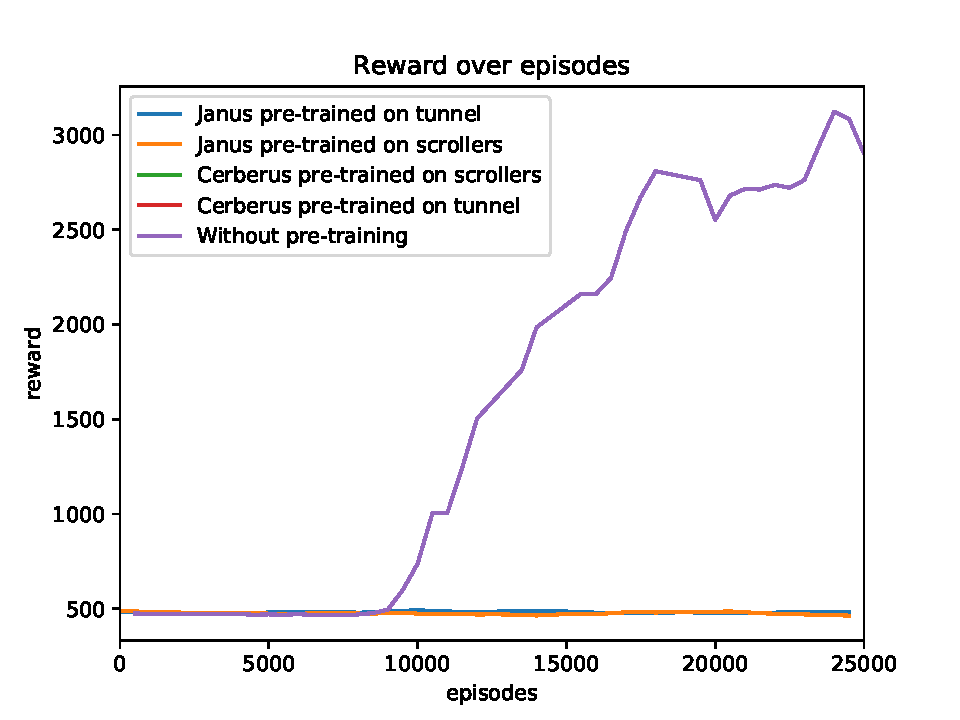
\includegraphics[width=\columnwidth]{img/rewards.pdf}
    \caption{Development of average rewards when training an agent for the Race task with either random initialization or pre-trained on Tunnel/Scrollers using Janus/Cerberus.}
    \label{fig:improved-learning}
\end{figure}
\section{Discussion}
\label{sec:discussion}
%\lipsum[2-3]
\subsection{Related Work}


\section{Conclusion}
\label{sec:conclusion}

% summary approach
In this work, we proposed a novel approach to automatic transfer learning in the domain of reinforcement learning on visual tasks. Our model builds on the DDQN architecture \citep{DDQN} that uses convolutional layers to transform the input images into a latent space. We add an additional representation module that is supposed to guide the latent space to more generalizable representations. To do so, the representation module additionally updates the convolutional encoder based on an autoencoder loss, perceived from reconstructing the input states, predicting following states and/or predicting dynamics in the environment.

% summary key findings
Our results show that the proposed encoder architecture is not sufficient for constructing latent representations useful for inter-task transfer. Indeed, the pre-training on tasks makes learning more difficult for the agent than a random initialization. Furthermore, a detailed analysis of the latent space revealed it to lack focus on features relevant to the tasks. Particularly, the reconstruction loss favored global structures over local information, which made operating in some environments difficult for the agent.

\subsection{Future Work}
\label{subsec:futurework}
Overall, the experiment results reveal the general difficulty of creating a latent space that can facilitate knowledge transfer across RL tasks.
With multi-task learning on Scroller tasks, the latent space visualization shows that the states from some tasks are separated, indicating that knowledge transfer can hardly occur.
While this could be partially due to the chosen tasks lacking sufficient similarity, further extensions can be made to our framework in order to incentivize the merge of domains, for example by the adversarial domain classifier structure proposed by \citet{ganin2014unsupervised}.

Moreover, as our policy learner is a DDQN, it would be interesting to extend it to more advanced policy networks, such as Rainbow \citep{rainbow} or hierarchical-DQN \citep{hierarchical_dqn}.
Furthermore, additional convolutional layers may be helpful for constructing a meaningful latent space. 
%Since our results are promising it would be interesting to see our framework applied to Atari games.

Lastly, the DQN approach is using function approximation to learn a policy. That is, it tries to approximate Q-values. An alternative to this approach, so called policy gradient methods such as the REINFORCE algorithm \citep{williams1992simple} and its variations, could make learning and ultimately transferring easier, since the agent does not need to learn to approximate a Q-function. Instead, it directly learns the policy.


{\tiny\printbibliography}

\clearpage
\raggedbottom
\appendix
\begin{appendix}
\end{appendix}

\end{document}